%\documentclass[12pt,aspectratio=169]{beamer}
\documentclass[12pt]{beamer}

\usepackage[frenchb]{babel}
\usepackage[T1]{fontenc}
\usepackage[utf8]{inputenc}

\usepackage{pgfpages}

\usepackage{tikz}
\usetikzlibrary{arrows}
\usetikzlibrary{shapes}
\usetikzlibrary{trees}

\usepackage[pangram]{blindtext}

\usepackage[lang=fr]{templateLAAS}
\usepackage{amsmath}
\usepackage{multimedia}
\usepackage{xunicode,xltxtra}

\usepackage{tikz}
\usetikzlibrary{arrows}
\usetikzlibrary{calc}

\usepackage{cancel}

\usepackage{pgffor}
\usepackage{filecontents}% Used so that the external files can be placed in this file


%\setbeameroption{show notes}
%\setbeameroption{show notes on second screen=right}

\AtBeginSection[]
{
  {\canvasspecial
  \begin{frame}
  \frametitle{Sommaire}
  \tableofcontents[currentsection, hideothersubsections]
  \end{frame}}
}

\newcommand*{\vcenteredhbox}[1]{\begingroup
\setbox0=\hbox{#1}\parbox{\wd0}{\box0}\endgroup}


\title{TransHumUs}
\subtitle{Le projet français de la biennale de Venise 2015: \\Faire bouger trois arbres}
\author{Guilhem Saurel}
\institute{Gepetto}
\date{2 juin 2015}
%\titlegraphic{\includegraphics[height=2cm,keepaspectratio]{UT-UPS-LAAS}}

\begin{document}
    {\canvasspecial
    \begin{frame}
    \titlepage
    \end{frame}}

    \section{Présentation}
        \subsection{La Biennale de Venise}
            \begin{frame}{\subsecname: All The World’s Future}
                \begin{center}
                    
\includegraphics[width=3cm]{img/lion.jpg} \\
                    
\includegraphics[width=\linewidth]{img/ATWF4.png}
                \end{center}
            \end{frame}
            \begin{frame}{\subsecname: La Biennale dans Venise}
                \vspace{-0.4cm}
                \begin{center}
                    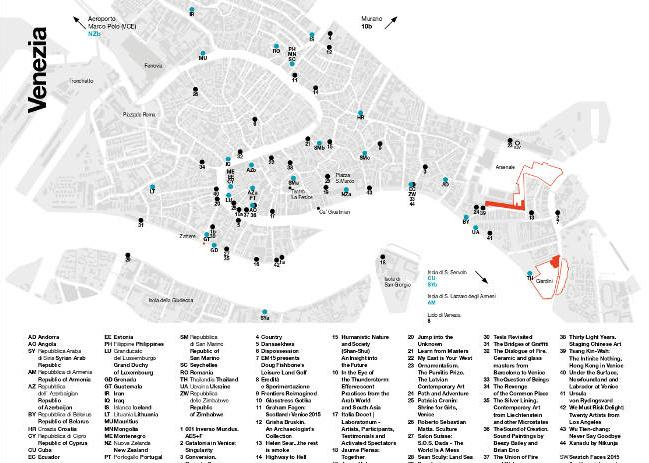
\includegraphics[height=8cm]{img/venise.jpg}
                \end{center}
            \end{frame}
            \begin{frame}{\subsecname: La Biennale aux Giardini}
                \vspace{-0.4cm}
                \begin{center}
                    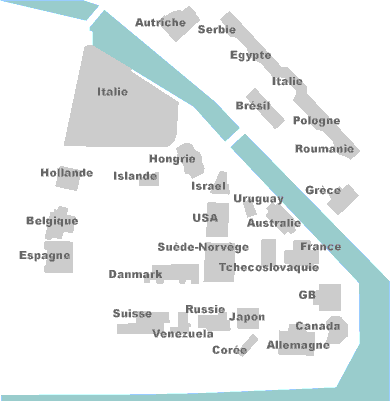
\includegraphics[height=8cm]{img/giardini.png}
                \end{center}
            \end{frame}
            \begin{frame}{\subsecname: Vue du ciel}
                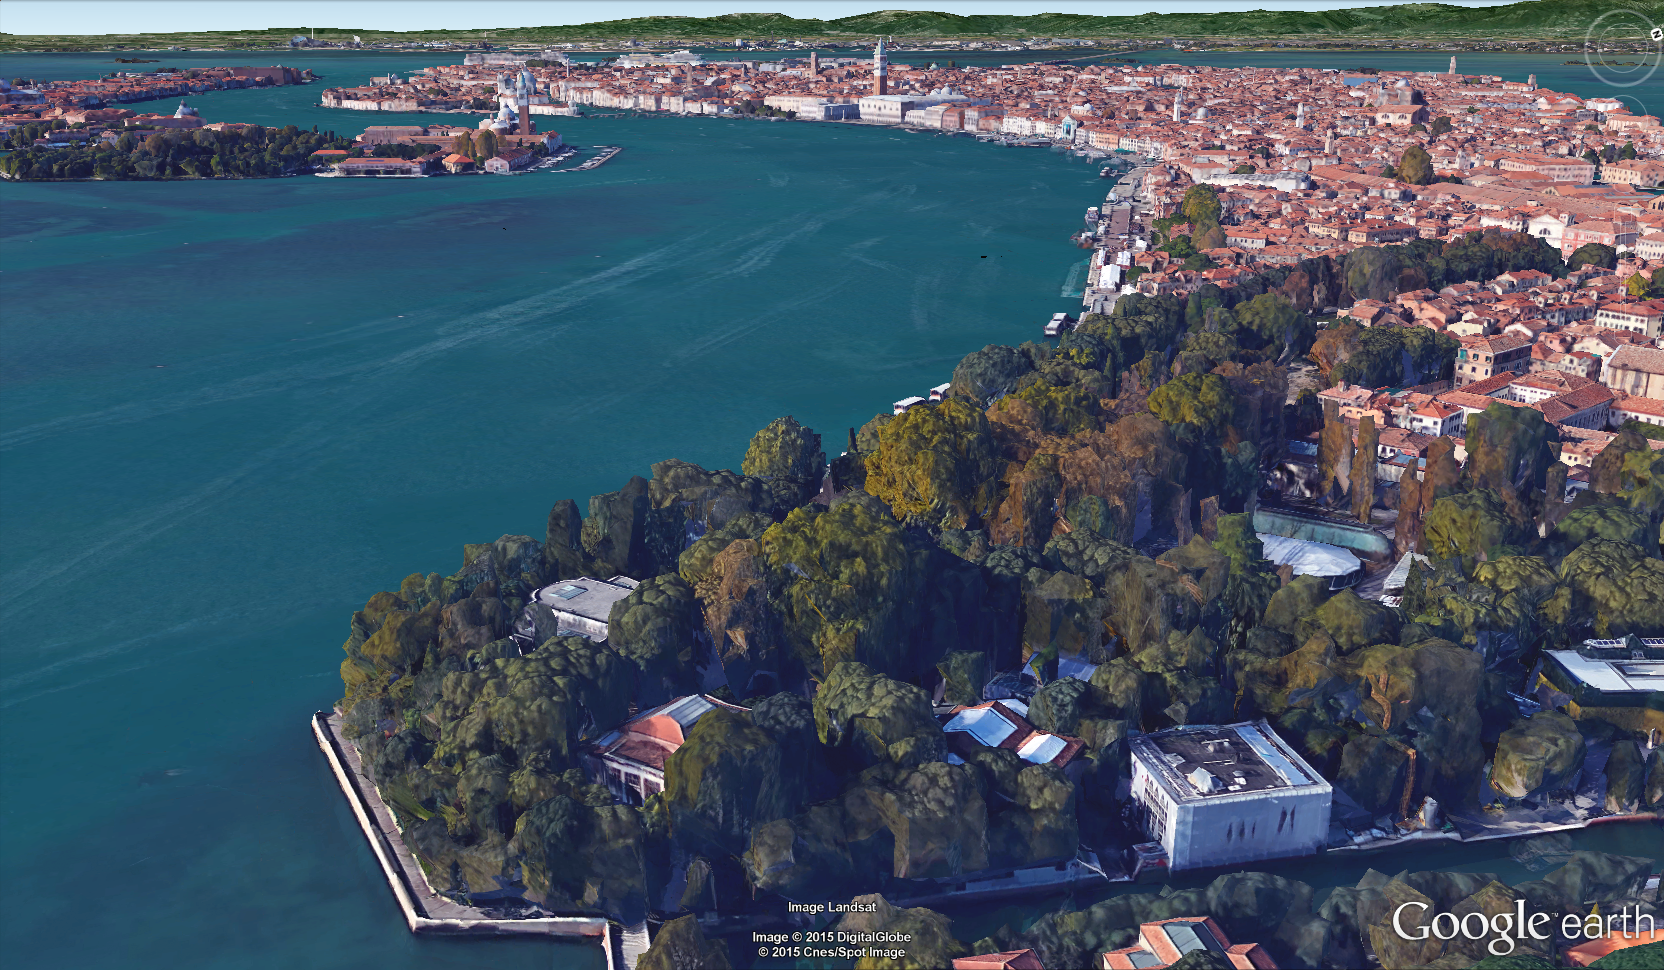
\includegraphics[width=\linewidth]{img/earth.png}
            \end{frame}
            \begin{frame}{\subsecname: Le Pavillon Français}
                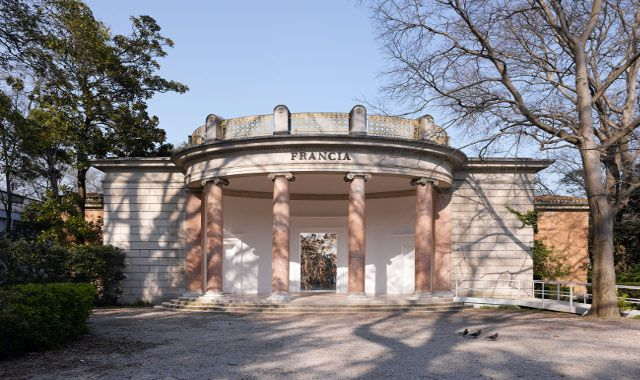
\includegraphics[width=\linewidth]{img/pavillon.jpg}
            \end{frame}

        \subsection{L’artiste}
            \begin{frame}{\subsecname: Céleste Boursier-Mougenot}
                \vspace{-0.4cm}
                \begin{center}
                    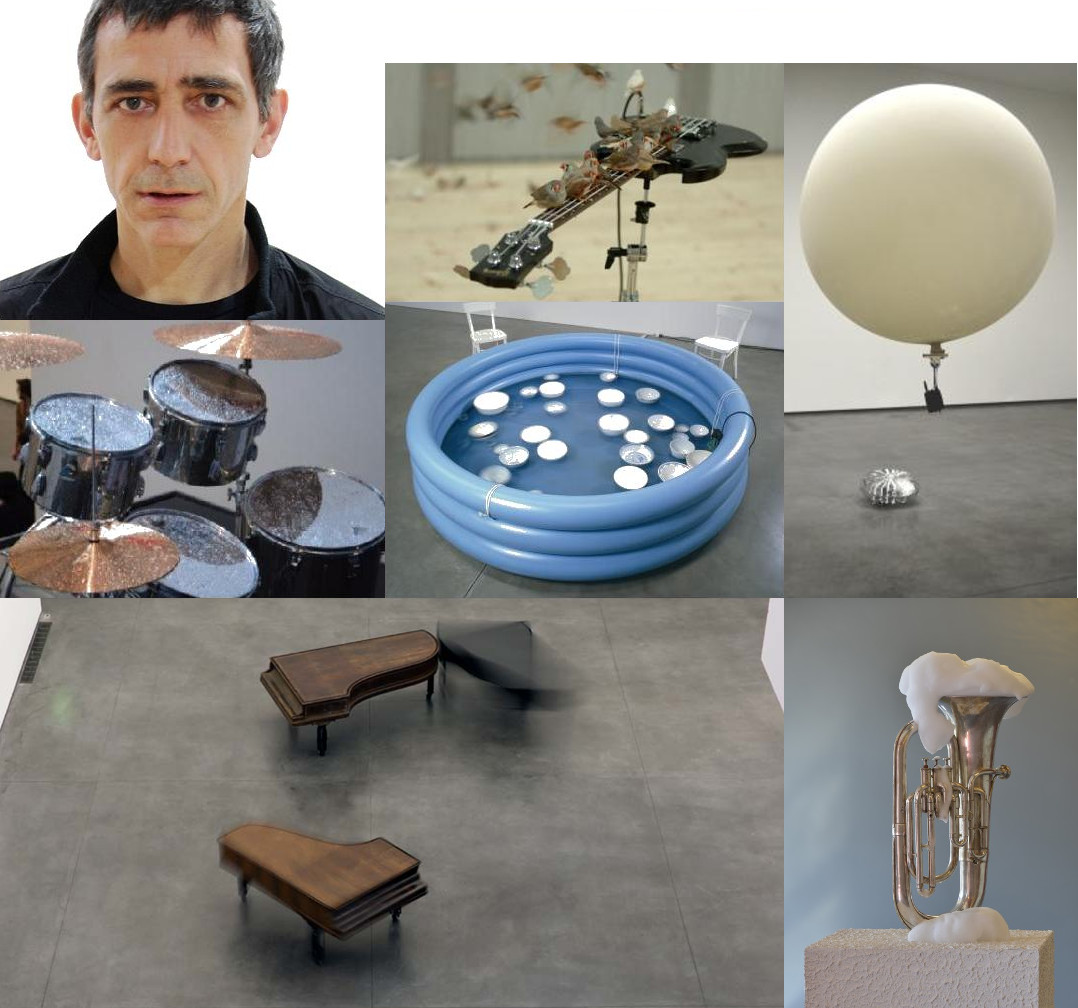
\includegraphics[height=8cm]{img/celeste2.jpg}
                \end{center}
            \end{frame}

        \subsection{Idée}
            \begin{frame}{\subsecname: \textit{Rêvolutions}, le projet artistique}
                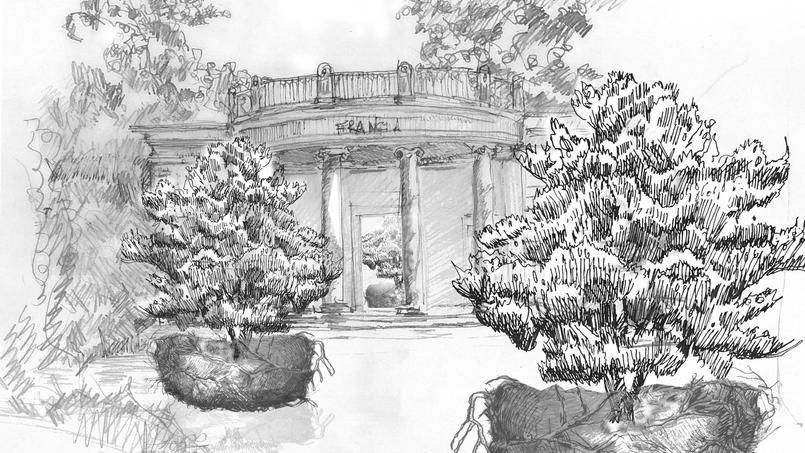
\includegraphics[width=\linewidth]{img/vue_artiste.jpg}
            \end{frame}

    \section{Rôle du LAAS}
        \subsection{Conseil Technique}
            {\canvasspecial
                \begin{frame}
                    \frametitle{Sommaire}
                \tableofcontents[hideothersubsections]
            \end{frame}}
            \subsubsection{Choix des prestataires}
                \begin{frame}{\subsubsecname: Base roulante}
                    Cahier des charges:
                    \begin{itemize}
                        \item 5 tonnes
                        \item 1 m/min et moins (5m/min en mode manuel)
                        \item h: 4.5m, \O: 2.5 m
                        \item Pas un bruit
                    \end{itemize}
                    10 Réponses à l’appel d’offre
                \end{frame}
                \begin{frame}{\subsubsecname: Automatic Guided Vehicles}
                    
\includegraphics[width=\linewidth]{img/ba.png}
                \end{frame}
                \begin{frame}{\subsubsecname: Livraison des AGV}
                    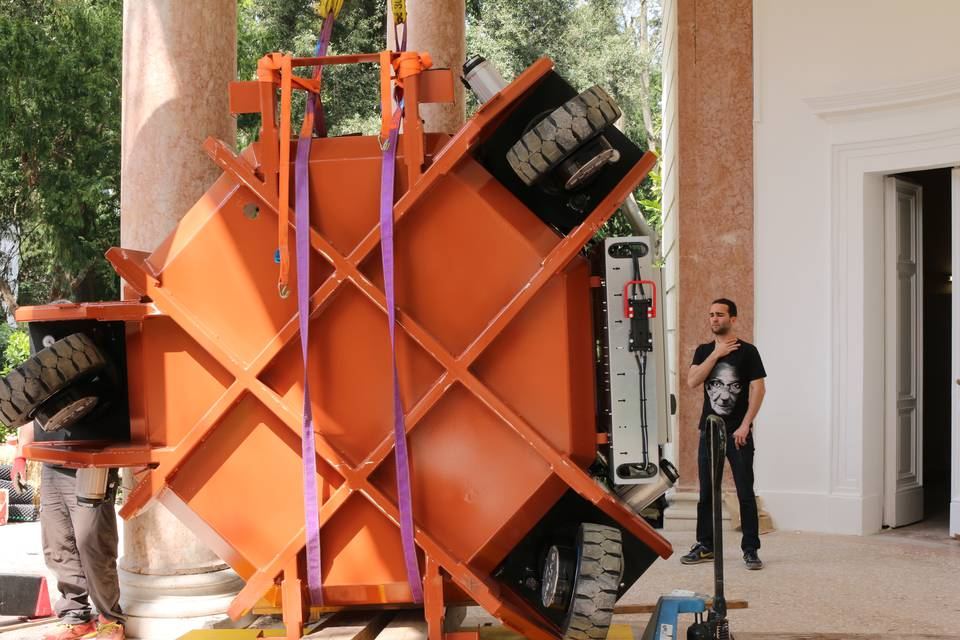
\includegraphics[width=\linewidth/3*2]{img/agv_vert.jpg}
                    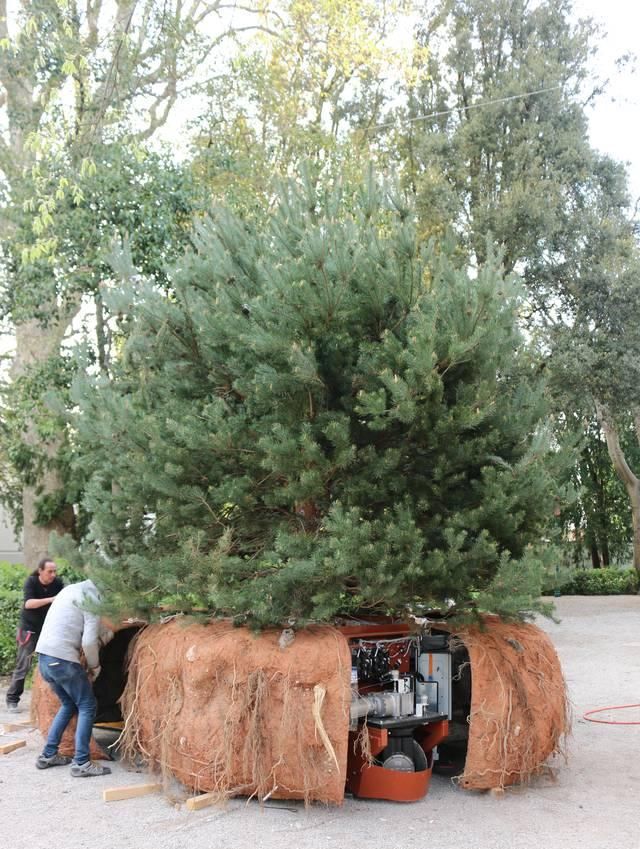
\includegraphics[width=\linewidth/3]{img/motte.jpg}
                \end{frame}
                \begin{frame}{\subsubsecname: Géolocalisation}
                    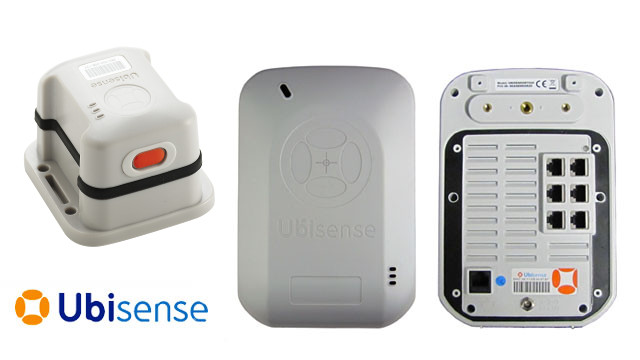
\includegraphics[width=\linewidth]{img/ubisense.jpg}
                \end{frame}
                %\begin{frame}{\subsubsecname: Sondes Granier}
                    %\vspace{-0.4cm}
                    %\begin{center}
                        %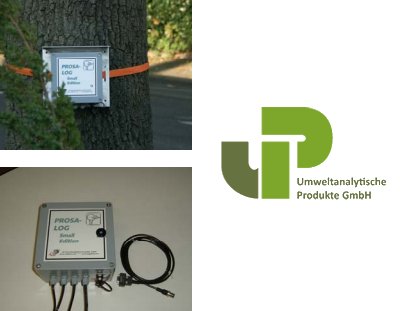
\includegraphics[height=8cm]{img/prosalog.png}
                    %\end{center}
                %\end{frame}

        \subsection{Conseil Scientifique}
            {\canvasspecial
                \begin{frame}
                    \frametitle{Sommaire}
                \tableofcontents[hideothersubsections]
            \end{frame}}
            \subsubsection{Lois du mouvement}
                \begin{frame}{\subsubsecname: Idée générale}
                    \begin{itemize}
                        \item Pas de sens privilégié
                        \item Mouvement holonome
                        \item 3 degrés de liberté → 3 variables d’entrée
                    \end{itemize}
                \end{frame}

            \subsubsection{Sondes Granier}
                \begin{frame}{\subsubsecname: Partenaires CNRS / UPS}
                    \begin{minipage}[t][1in][t]{3.5cm}\vspace{0pt}
                        Jérôme Chaves \\
                        
\includegraphics[width=3.5cm]{img/edb.jpg}
                    \end{minipage}
                    \begin{minipage}[t][1in][t]{3.5cm}\vspace{0pt}
                        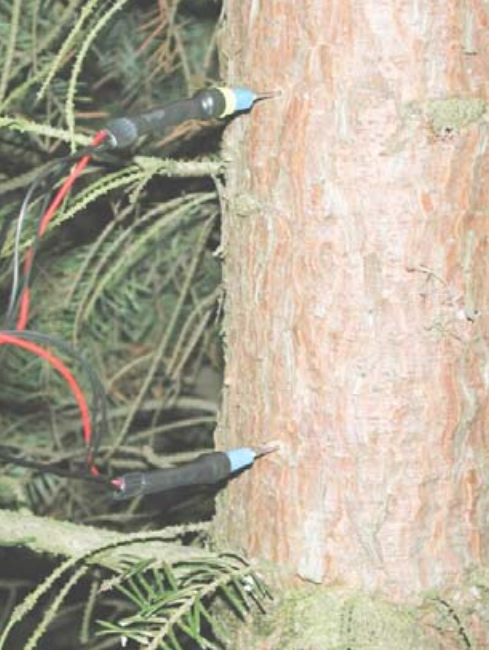
\includegraphics[width=3.5cm]{img/needles.png}
                    \end{minipage}
                    \begin{minipage}[t][1in][t]{3.5cm}\vspace{0pt}
                        Valérie Le Dantec \\
                        
\includegraphics[width=3.5cm]{img/cesbio.png}
                    \end{minipage}
                \end{frame}
                \begin{frame}{\subsubsecname: Expérimentations au LAAS}
                    \vspace{-0.5cm}
                    \begin{minipage}[t][1in][t]{3.5cm}\vspace{0pt}
                        Jérôme Chaves \\
                        
\includegraphics[width=3.5cm]{img/edb.jpg}
                    \end{minipage}
                    \begin{minipage}[t][1in][t]{3.5cm}\vspace{0pt}
                        
\includegraphics[width=3cm]{img/laas.png}
                    \end{minipage}
                    \begin{minipage}[t][1in][t]{3.5cm}\vspace{0pt}
                        Valérie Le Dantec \\
                        
\includegraphics[width=3.5cm]{img/cesbio.png}
                    \end{minipage}

                    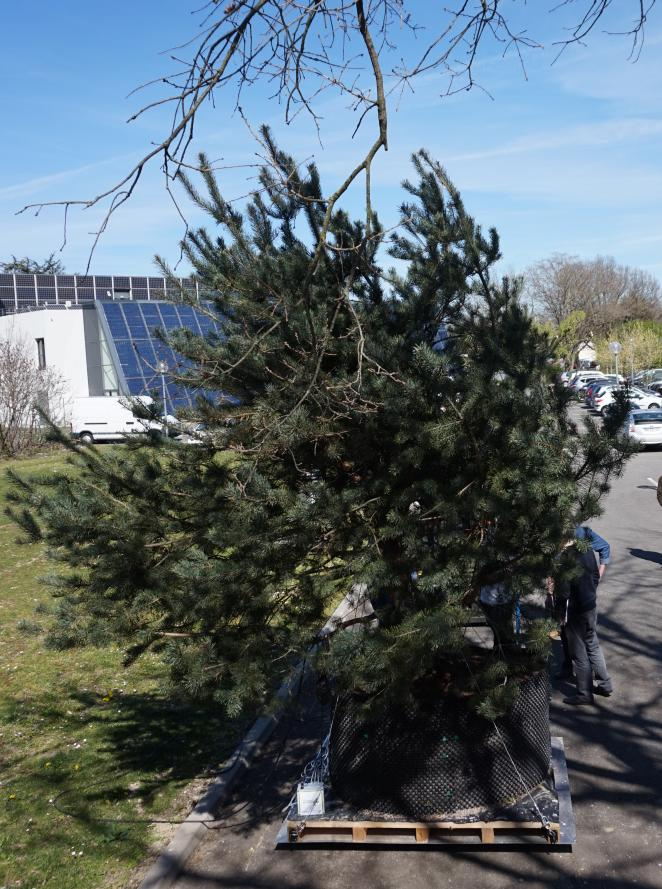
\includegraphics[width=3.5cm]{img/arbre_laas.jpg}
                    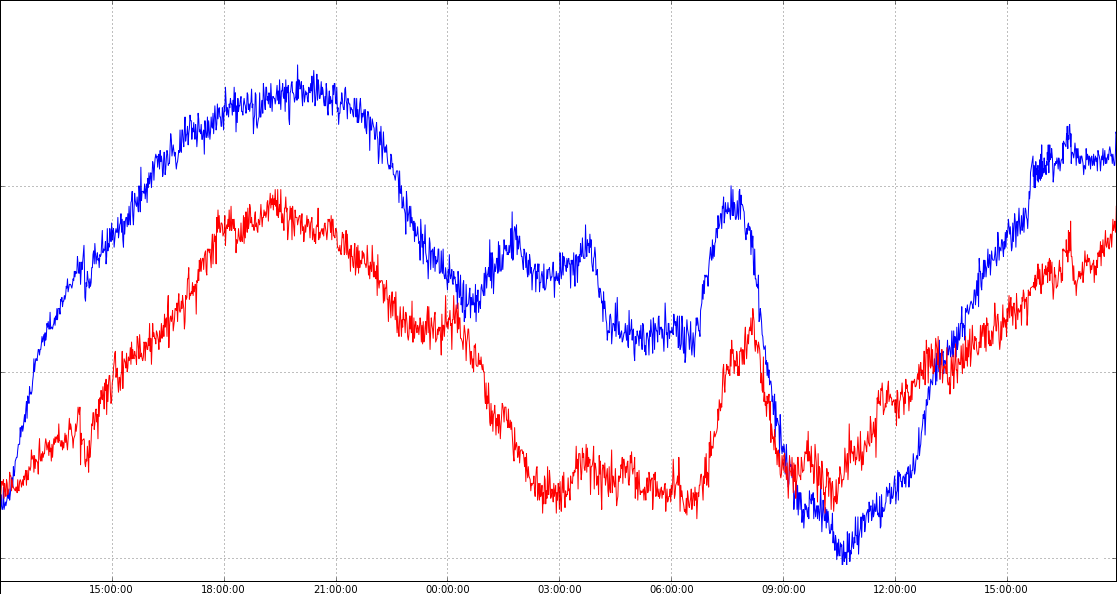
\includegraphics[width=7cm]{img/granier.png}
                \end{frame}

    \section{R\&D, définition du mouvement}
        \subsection{Définition du problème}
            \begin{frame}{\subsecname: Problématique Robotique}
                \begin{tikzpicture}
                    \draw
                    (0,0) node[text width=12cm, align=center, above] {\textbf{Espace Physique} ~~~~~~~~~~~~~~~~~~~~~~~~~~~~~~~~~~~~~~~~~~~~~~~~~~~~~~~~~~~~  Trajectoire lente, mouvement silencieux } --
                    (-3,-2) node[text width=6cm, align=center, below] {\textbf{Espace Sensoriel}
                                                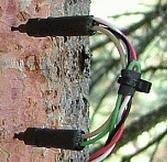
\includegraphics[width=1.7cm]{img/sapflow.jpg}
                                                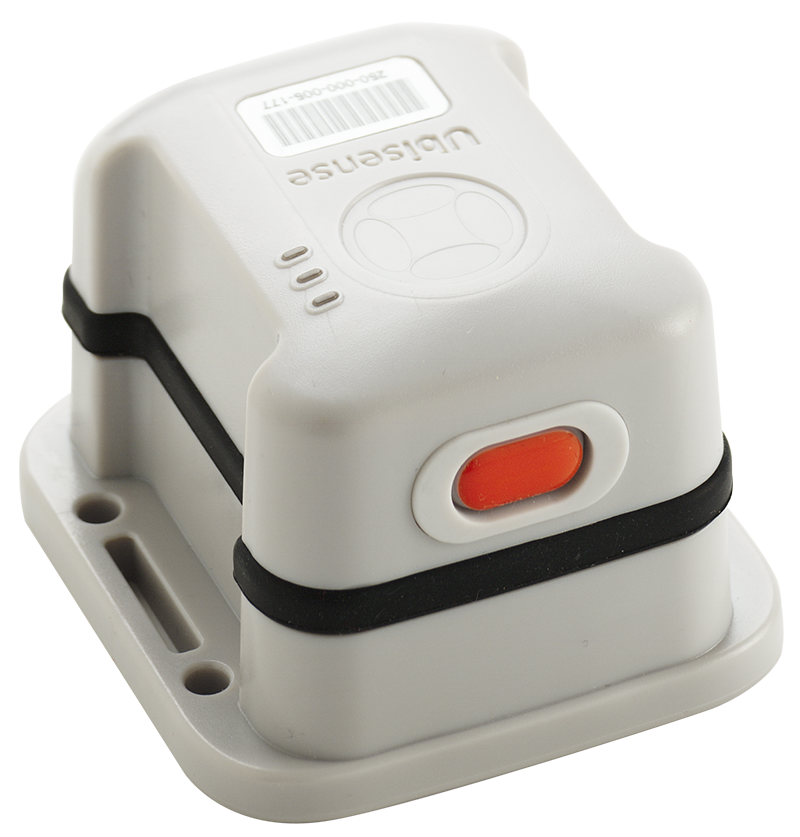
\includegraphics[width=1.7cm]{img/Ubisense-Tag.png}
                                                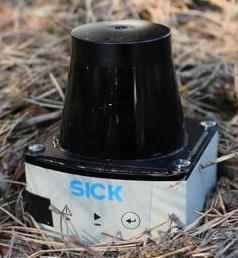
\includegraphics[width=1.7cm]{img/sick.jpg}
                                            } --
                    (3,-2) node[text width=6cm, align=center, below] {\textbf{Contrôle}
                                                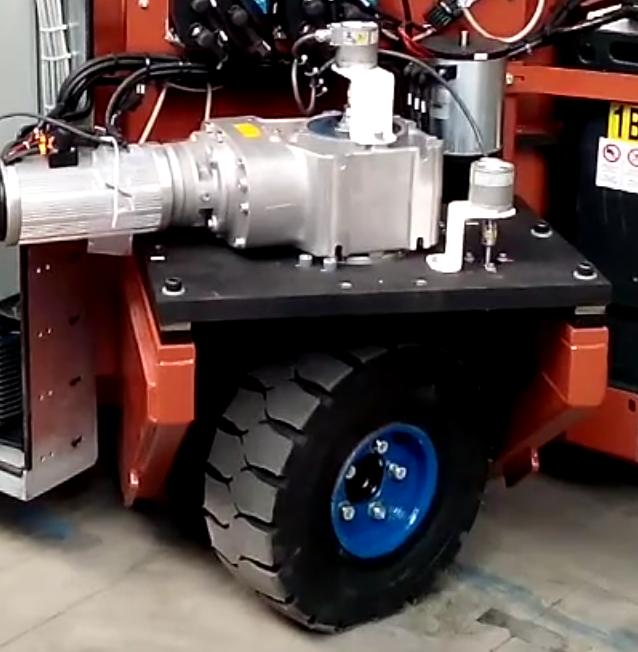
\includegraphics[width=1.7cm]{img/tourelle.jpg}
                                                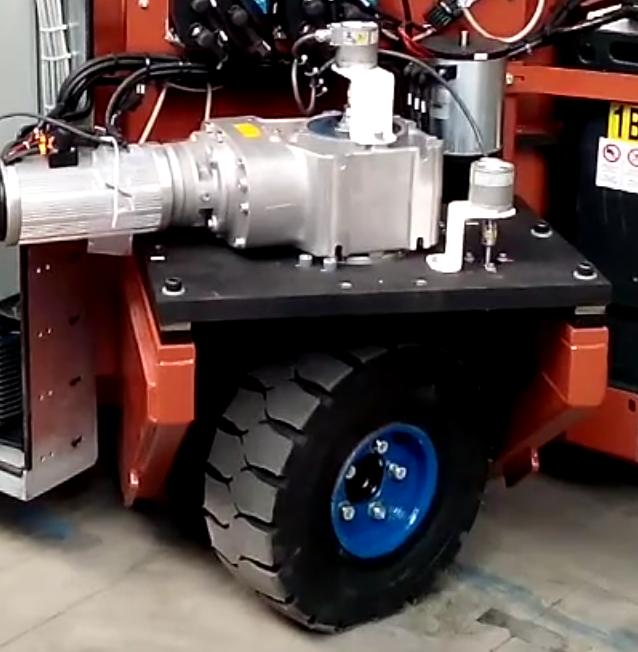
\includegraphics[width=1.7cm]{img/tourelle.jpg}
                                                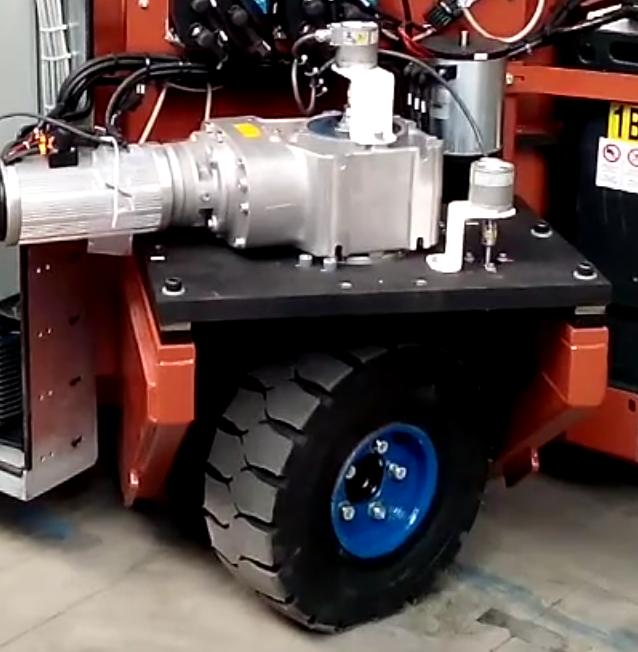
\includegraphics[width=1.7cm]{img/tourelle.jpg}
                                            } --
                    (0,0);
                \end{tikzpicture}
            \end{frame}
            \begin{frame}{\subsecname: Lieu}
                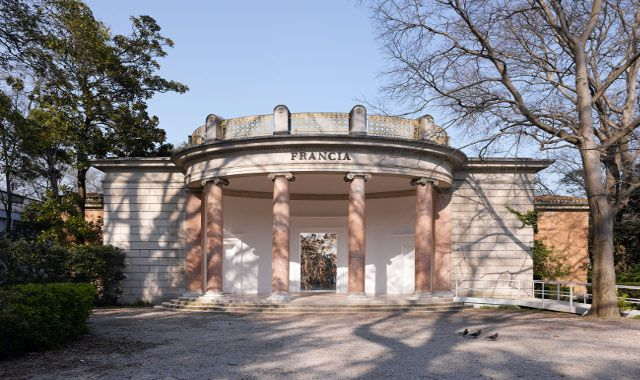
\includegraphics[width=\linewidth]{img/pavillon.jpg}
            \end{frame}
            \begin{frame}{\subsecname: Plan}
                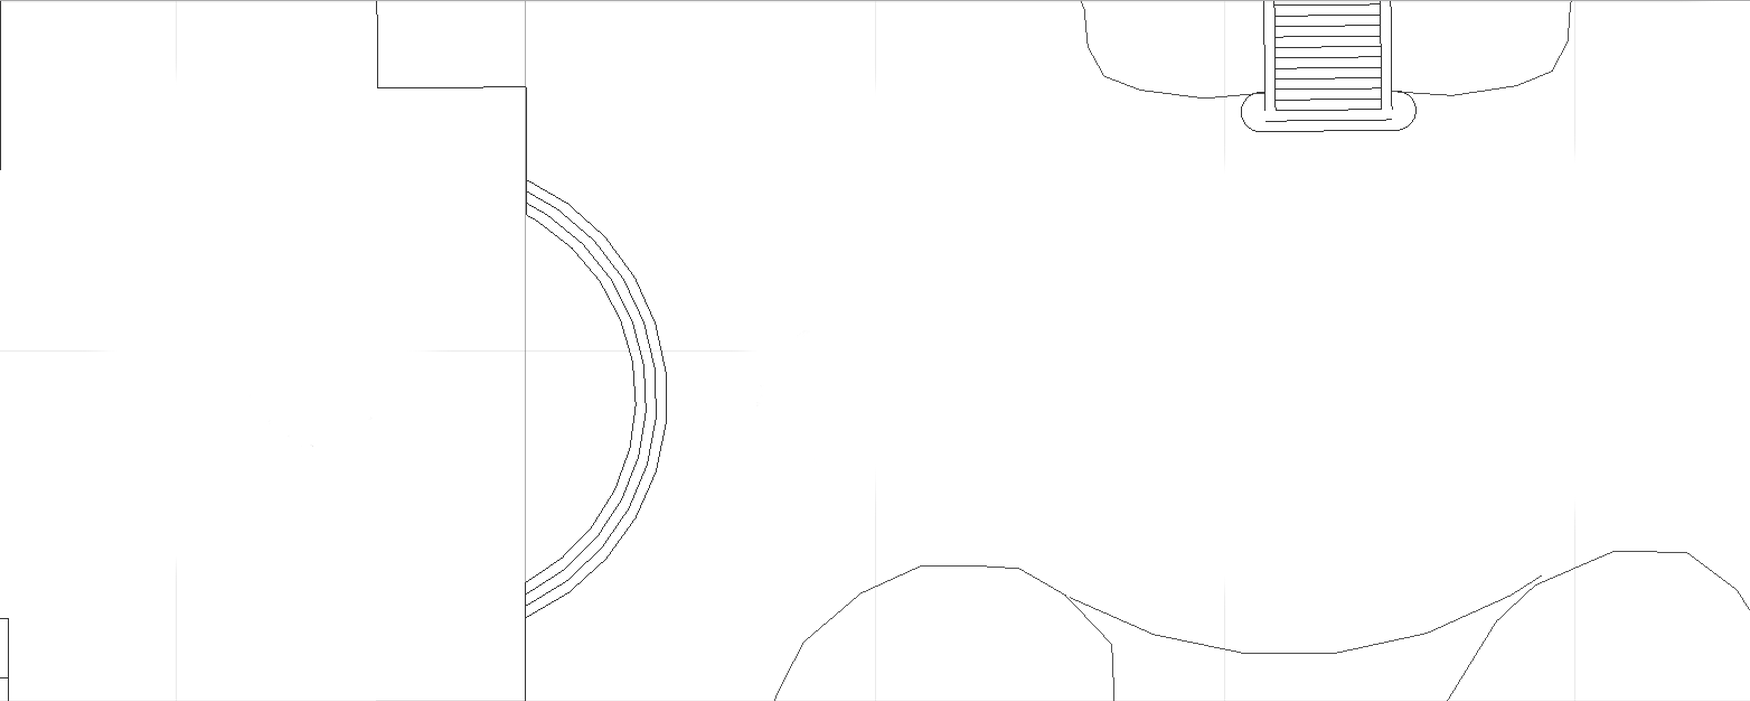
\includegraphics[width=\linewidth]{img/plan.png}
            \end{frame}
            \begin{frame}{\subsecname: Idée principale}
                \begin{itemize}
                    \item Un arbre à l’intérieur
                    \item Deux arbres à l’extérieur
                \end{itemize}
            \end{frame}
            \begin{frame}{\subsecname: Aire de jeu}
                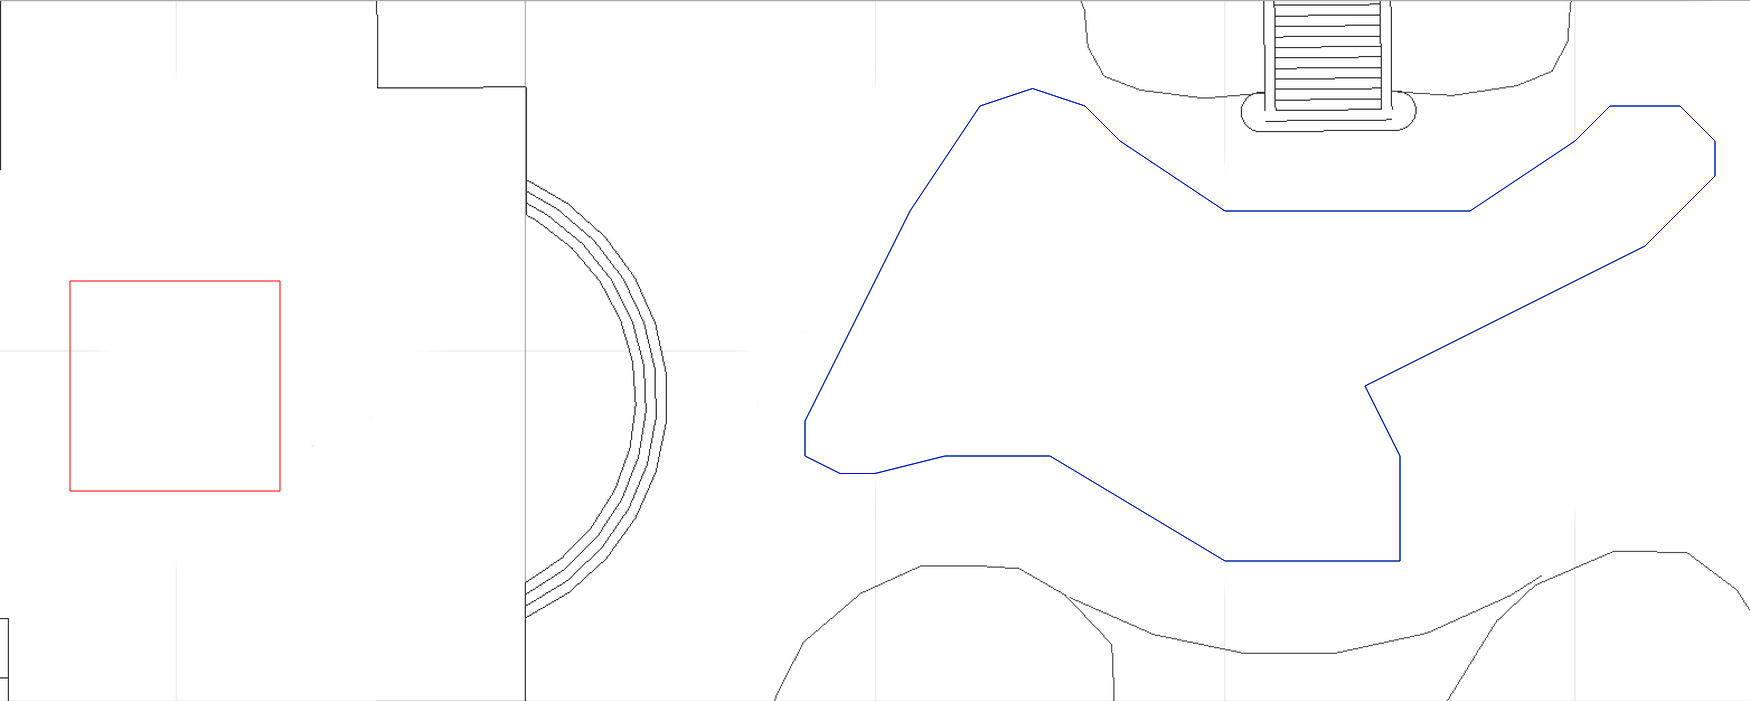
\includegraphics[width=\linewidth]{img/plan_bords.png}
            \end{frame}
        \subsection{Contrôle}
            \begin{frame}{\subsecname: AGV Tri-tourelles}
                \begin{itemize}
                    \item Sorties: $(v_i, \theta_i)$ Pour chaque tourelle
                    \item Entrées: $v$, $\omega$ \& $\theta$ Pour l’AGV
                \end{itemize}
                \begin{tikzpicture}
                    \draw (0, 0) node[draw,thick,minimum size=4cm,name=O,regular polygon,regular polygon sides=8] {};
                    \draw (O) node[circle,draw,inner sep=1pt] {};
                    \coordinate (a) at (O.side 2);
                    \coordinate (b) at (O.side 4);
                    \coordinate (c) at (O.side 7);
                    \draw (a) node[fill=red,circle,draw,inner sep=1pt] {};
                    \draw (b) node[fill=red,circle,draw,inner sep=1pt] {};
                    \draw (c) node[fill=red,circle,draw,inner sep=1pt] {};
                \end{tikzpicture}
            \end{frame}
            \begin{frame}{\subsecname: AGV Tri-tourelles}
                \begin{itemize}
                    \item Sorties: $(v_i, \theta_i)$ Pour chaque tourelle
                    \item Entrées: $v$, $\omega$ \& $\theta$ Pour l’AGV
                \end{itemize}
                \begin{tikzpicture}
                    \draw (0, 0) node[draw,thick,minimum size=4cm,name=O,regular polygon,regular polygon sides=8] {};
                    \draw (O) node[circle,draw,inner sep=1pt] {};
                    \coordinate (a) at (O.side 2);
                    \coordinate (b) at (O.side 4);
                    \coordinate (c) at (O.side 7);
                    \draw (a) node[fill=red,circle,draw,inner sep=1pt] {};
                    \draw (b) node[fill=red,circle,draw,inner sep=1pt] {};
                    \draw (c) node[fill=red,circle,draw,inner sep=1pt] {};
                    \draw[->, red] (0, 0) -- (0.5,0.866);
                    \draw[red] (0, 0.5) node {$v$};
                    \draw[->, red] (a) -- ($ (a) + (0.5,0.866) $);
                    \draw[->, red] (b) -- ($ (b) + (0.5,0.866) $);
                    \draw[->, red] (c) -- ($ (c) + (0.5,0.866) $);
                    \node (origin) at (0,0) {};
                    \node (xaxis) at (0:1) {};
                    \node (avector) at (60:1) {};
                    \draw[opacity=0] (origin) -- coordinate (va) (xaxis);
                    \draw[opacity=0] (origin) -- coordinate (vb) (avector);
                    \tikzset{angle/.style={bend right}}
                    \draw[angle,->] (va) to node[above] {$\theta$} (vb);
                \end{tikzpicture}
                Pour $v=1$, $\theta=\pi/3$, $\omega=0$
            \end{frame}
            \begin{frame}{\subsecname: AGV Tri-tourelles}
                \begin{itemize}
                    \item Sorties: $(v_i, \theta_i)$ Pour chaque tourelle
                    \item Entrées: $v$, $\omega$ \& $\theta$ Pour l’AGV
                \end{itemize}
                \begin{tikzpicture}
                    \draw (0, 0) node[draw,thick,minimum size=4cm,name=O,regular polygon,regular polygon sides=8] {};
                    \draw (O) node[fill=green,circle,draw,inner sep=1pt] {};
                    \coordinate (a) at (O.side 2);
                    \coordinate (b) at (O.side 4);
                    \coordinate (c) at (O.side 7);
                    \draw (a) node[fill=red,circle,draw,inner sep=1pt] {};
                    \draw (b) node[fill=red,circle,draw,inner sep=1pt] {};
                    \draw (c) node[fill=red,circle,draw,inner sep=1pt] {};
                    \draw[->, green] (a) -- ($ (a) + (-0.707,-0.707) $);
                    \draw[->, green] (b) -- ($ (b) + (+0.707,-0.707) $);
                    \draw[->, green] (c) -- ($ (c) + (0,1) $);
                \end{tikzpicture}
                Pour $v=0$, $\omega=1$
            \end{frame}
            \begin{frame}{\subsecname: AGV Tri-tourelles}
                \begin{itemize}
                    \item Sorties: $(v_i, \theta_i)$ Pour chaque tourelle
                    \item Entrées: $v$, $\omega$ \& $\theta$ Pour l’AGV
                \end{itemize}
                \begin{tikzpicture}
                    \draw (0, 0) node[draw,thick,minimum size=4cm,name=O,regular polygon,regular polygon sides=8] {};
                    \draw (O) node[fill=green,circle,draw,inner sep=1pt] {};
                    \coordinate (a) at (O.side 2);
                    \coordinate (b) at (O.side 4);
                    \coordinate (c) at (O.side 7);
                    \draw (a) node[fill=red,circle,draw,inner sep=1pt] {};
                    \draw (b) node[fill=red,circle,draw,inner sep=1pt] {};
                    \draw (c) node[fill=red,circle,draw,inner sep=1pt] {};
                    \draw[->, red] (0, 0) -- (0.5,0.866);
                    \draw[->, red] (a) -- ($ (a) + (0.5,0.866) $);
                    \draw[->, red] (b) -- ($ (b) + (0.5,0.866) $);
                    \draw[->, red] (c) -- ($ (c) + (0.5,0.866) $);
                    \draw[->, green] (a) -- ($ (a) + (-0.707,-0.707) $);
                    \draw[->, green] (b) -- ($ (b) + (+0.707,-0.707) $);
                    \draw[->, green] (c) -- ($ (c) + (0,1) $);
                    \draw[->] (a) -- ($ (a) + (0.5,0.866) + (-0.707,-0.707) $);
                    \draw[->] (b) -- ($ (b) + (0.5,0.866) + (+0.707,-0.707) $);
                    \draw[->] (c) -- ($ (c) + (0.5,0.866) + (0,1) $);
                \end{tikzpicture}
                Pour $v=1$, $\theta=\pi/3$, $\omega=1$
            \end{frame}

            \begin{frame}{\subsecname: AGV Tri-tourelles}
                \begin{itemize}
                    \item Sorties: $(v_i, \theta_i)$ Pour chaque tourelle
                    \item Entrées: $v$, $\omega$ \& $\theta$ Pour l’AGV
                    \item Donc par tourelle:
                        \begin{eqnarray*}
                            v_{xi} &=& v \cos(\theta)- \omega \sin(\alpha_i) \\
                            v_{yi} &=& v \sin(\theta)+ \omega \cos(\alpha_i) \\
                            v_i &=& \sqrt{v_{xi}^2 + v_{yi}^2} \\
                            \theta_i &=& \arctan(v_{yi}, v_{xi})
                        \end{eqnarray*}
                    \item Centre instantané de rotation unique
                \end{itemize}
            \end{frame}
        \subsection{Trajectoires}
            \begin{frame}{\subsecname: Destination}
                \begin{itemize}
                    \item L’arbre est en $(x, y, \alpha)$ et veut rejoindre $(x_G, y_G)$
                    \item Il y va en fontion de ses sondes Granier $(g_1, g_2, g_3)$:
                        \begin{eqnarray*}
                            v &=& f_v(g_1) \in [0, 1] \\
                            \omega &=& f_\omega(g_2) \in [-1, 1] \\
                            \theta &=& \arctan(y - y_G, x - x_G) - \alpha + f_\theta(g_3)
                        \end{eqnarray*}
                \end{itemize}
            \end{frame}
            \begin{frame}{\subsecname: Choix de la destination}
                \begin{itemize}
                    \item L’arbre enregistre l’ensoleillement moyen qu’il perçoit en fonction du lieu
                    \item Il alterne ensuite entre un point ensoleillé, un point à l’ombre, et un point inconnu
                    \item Lorsque les arbres extérieurs sont trop près l’un de l’autre, ils retournent au cœur du polygone étoilé pour avoir la place de manœuvrer
                \end{itemize}
            \end{frame}

    \section{Intégration}
        \subsection{Framework}
            \begin{frame}{\subsecname: Simulateur}
                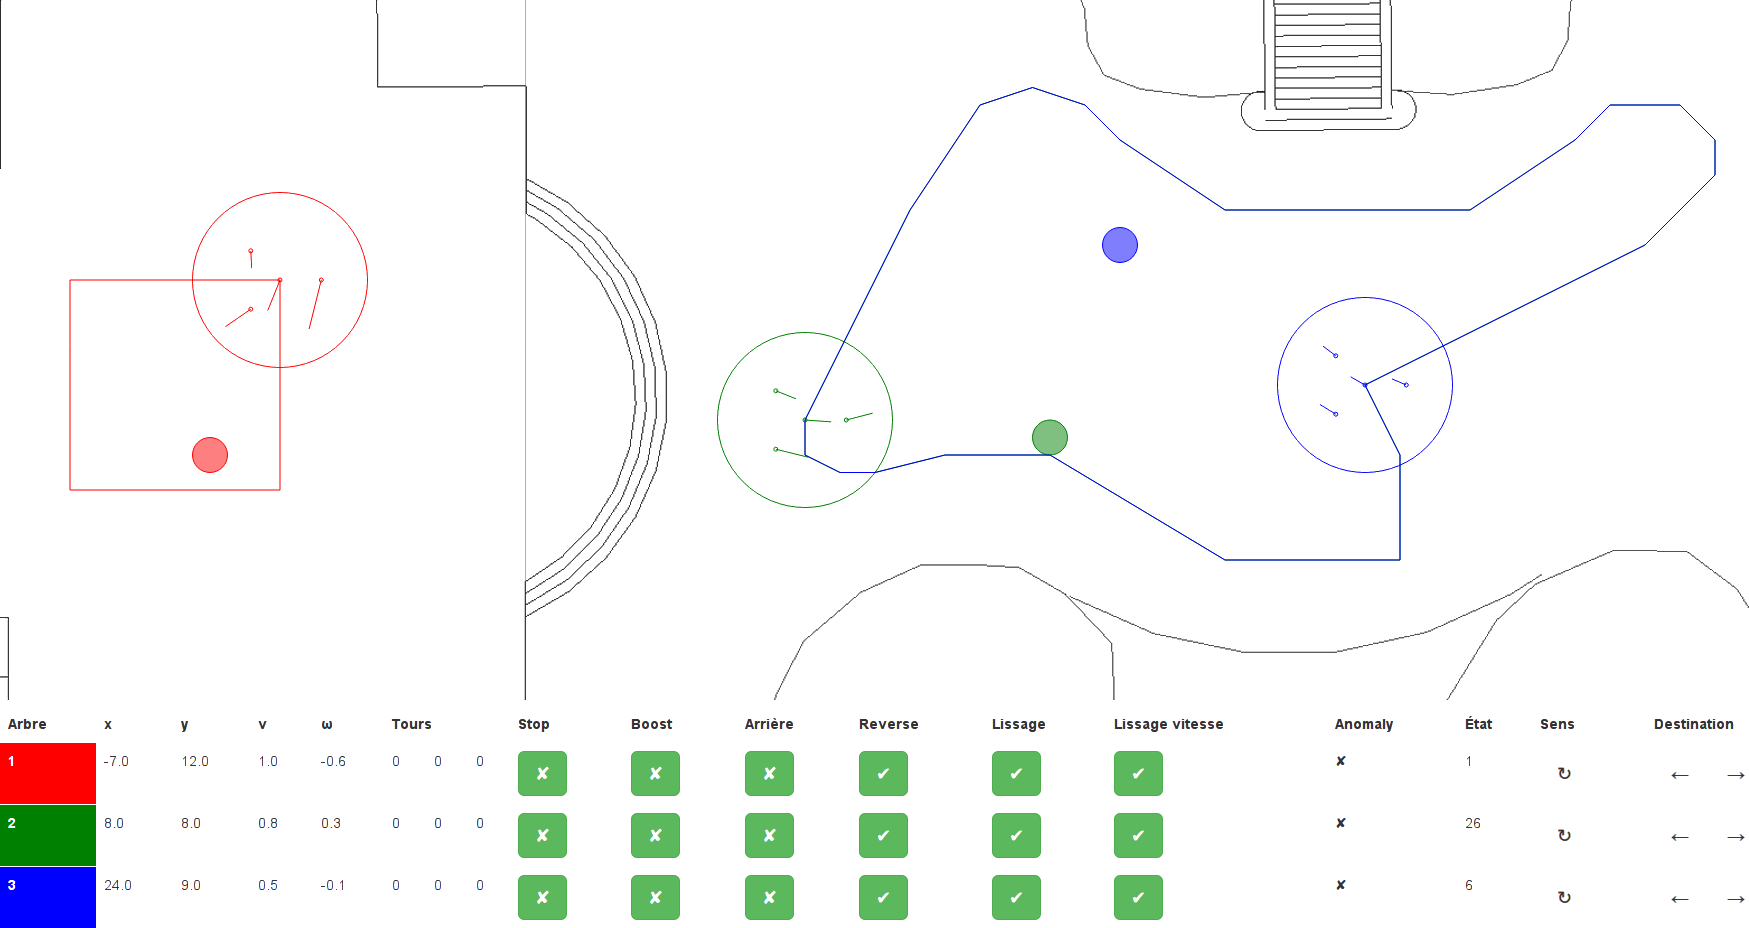
\includegraphics[width=\linewidth]{img/simu.png}
            \end{frame}
        \subsection{Géolocalisation}
            \begin{frame}{\subsecname: Placement des antennes}
                \vspace{-0.4cm}
                \begin{center}
                    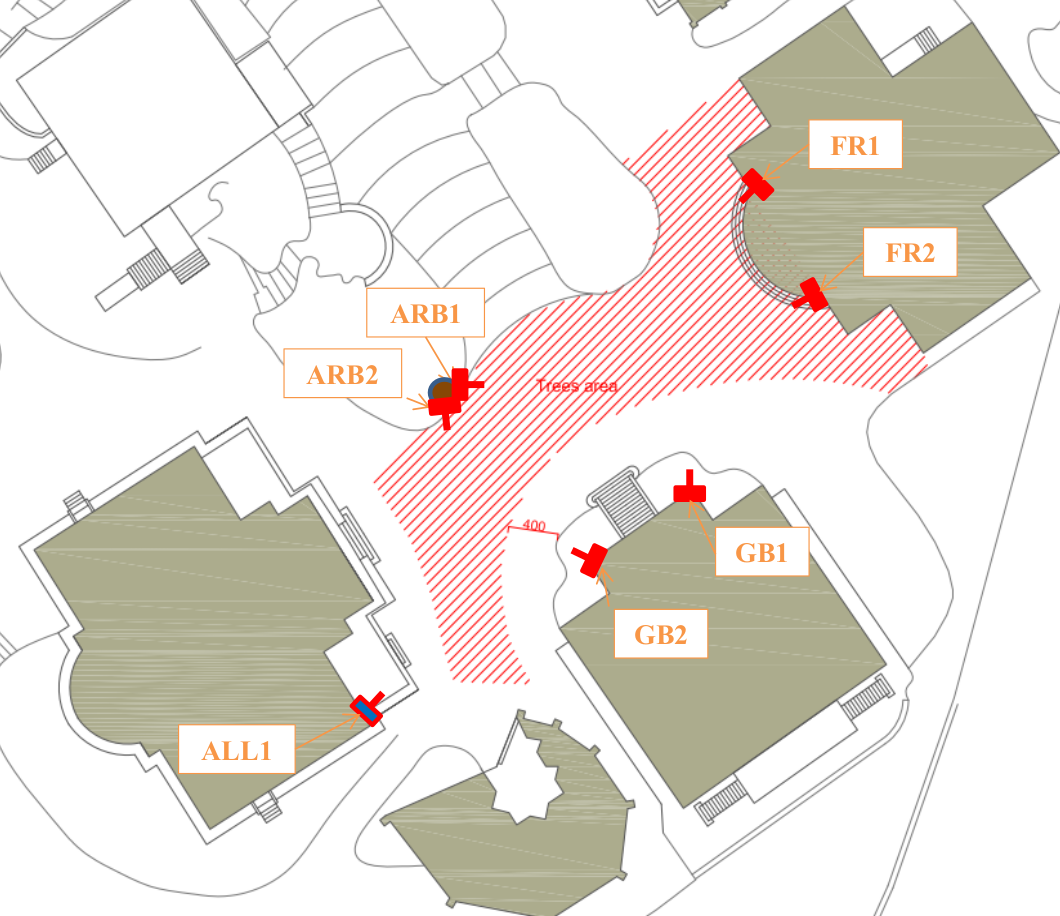
\includegraphics[height=8cm]{img/antennes.png}
                \end{center}
            \end{frame}
            \begin{frame}{\subsecname: Précision}
                \begin{center}
                    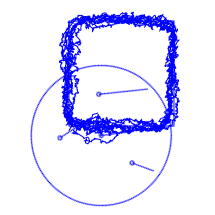
\includegraphics[height=3cm]{img/carre_ok.png} \pause
                    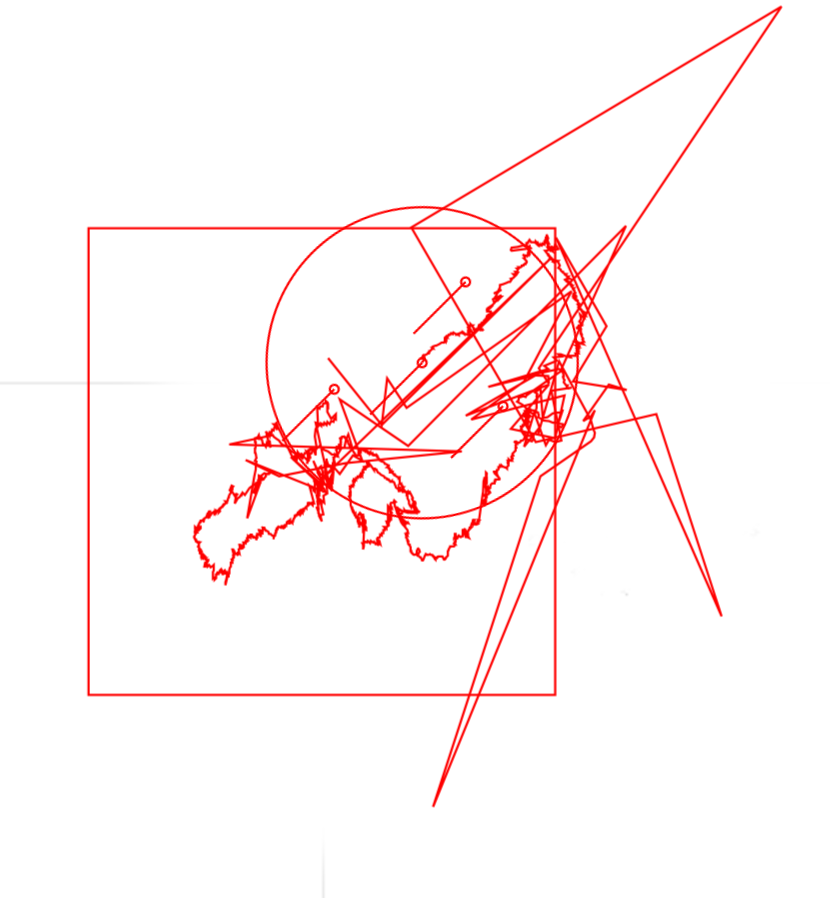
\includegraphics[height=3cm]{img/carre_ko.png}
                \end{center}
            \end{frame}
        \subsection{Contrôle}
            \begin{frame}{\subsecname: Limites des capacités des AGV}
                \begin{block}{Glissements}
                    Les roues en caoutchouc crissent sur le sol intérieur en tournant → Il faut éloigner les CIR des roues
                \end{block}
                \begin{block}{Vitesse}
                    La vitesse limite basse est finalement beaucoup plus haute que prévu → On reste à 1 m/min tout le temps
                \end{block}
            \end{frame}
            \begin{frame}{\subsecname: Embourbement}
                \begin{center}
                    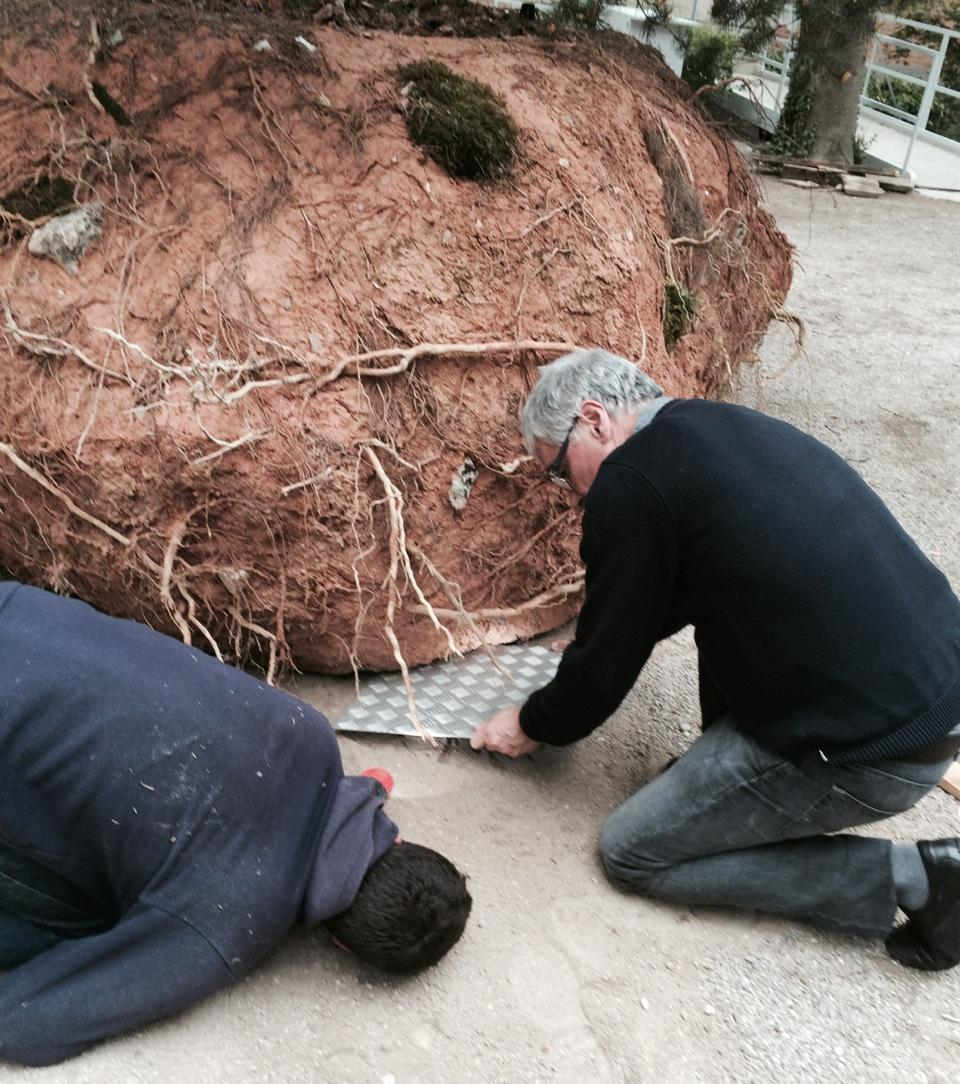
\includegraphics[height=7cm]{img/embourbemenet.jpg}
                    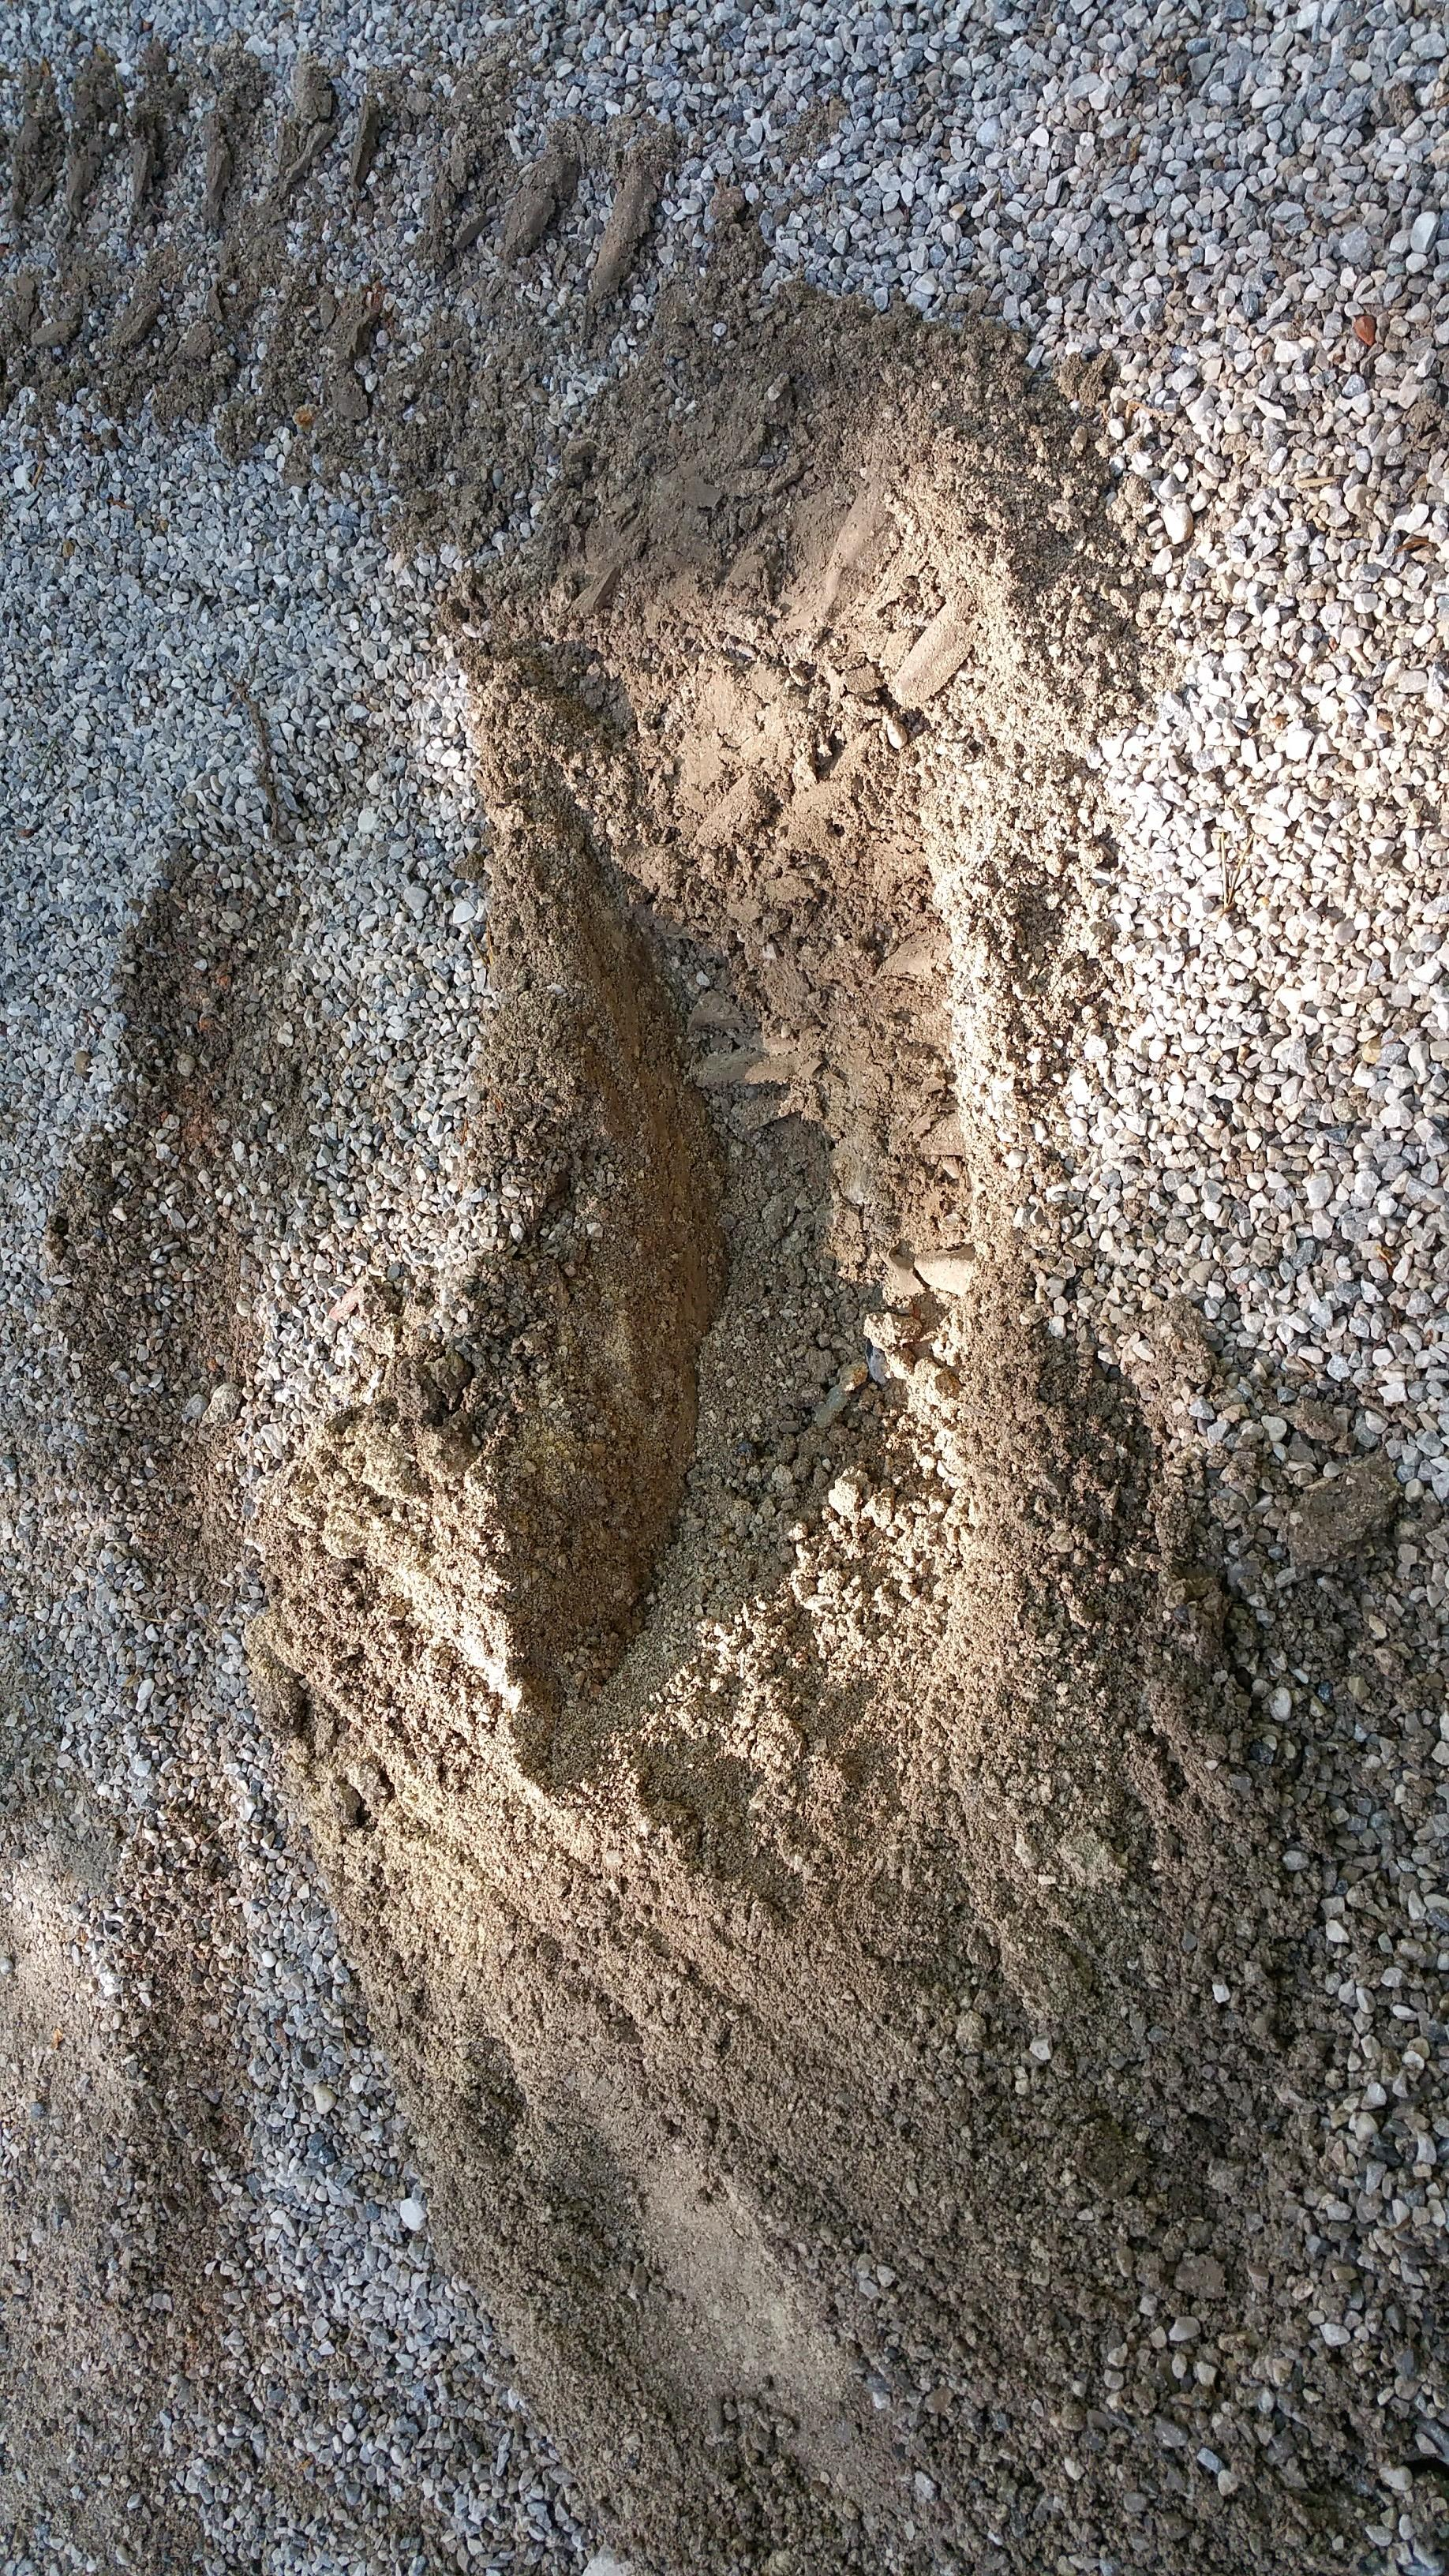
\includegraphics[height=7cm]{img/embourbe.jpg}
                \end{center}
            \end{frame}
        \subsection{Trajectoires}
            \begin{frame}{\subsecname}
                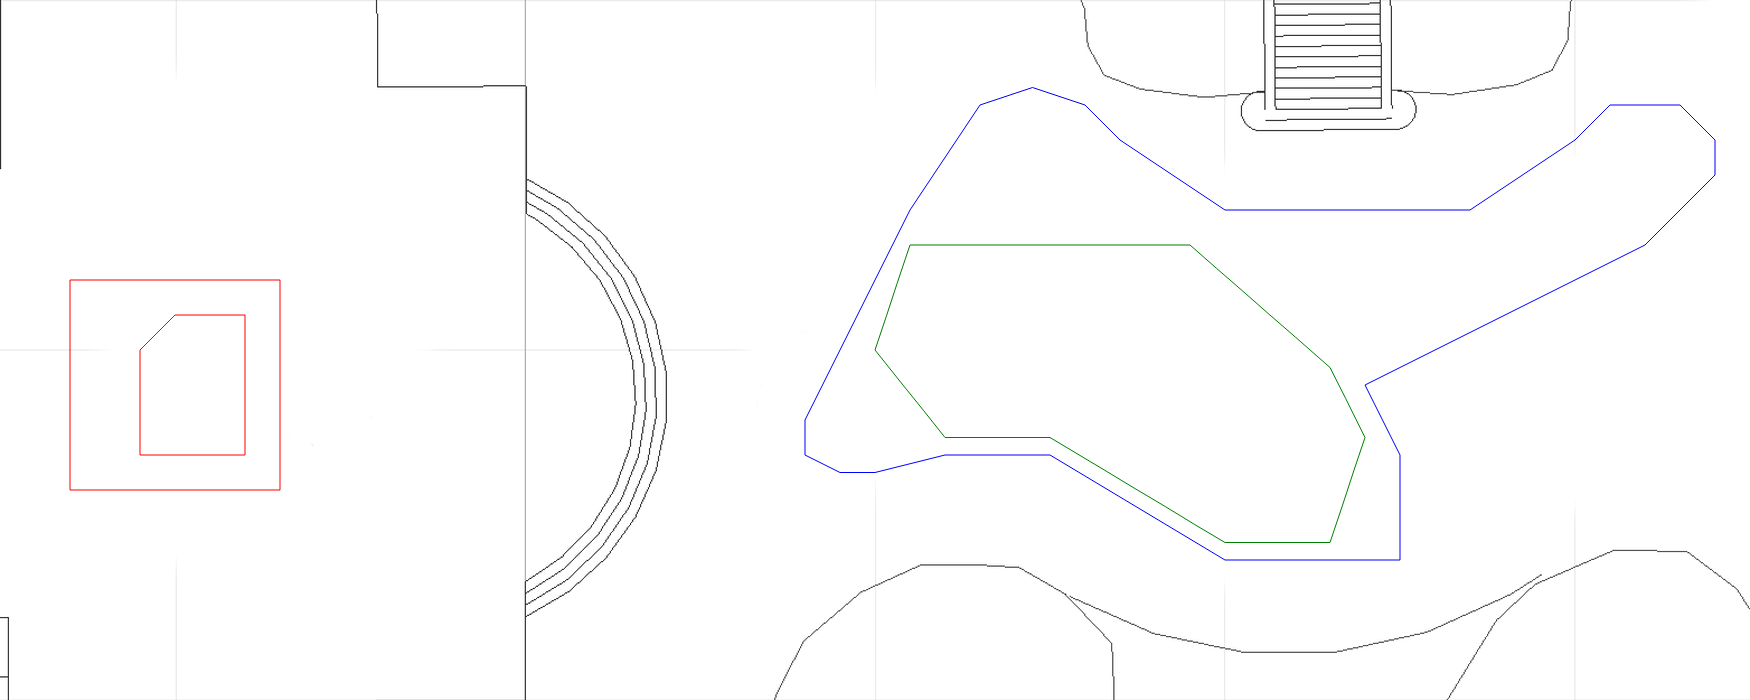
\includegraphics[width=\linewidth]{img/boucles.png}
            \end{frame}
            \begin{frame}{\subsecname: Destination}
                \begin{itemize}
                    \item L’arbre est en $(x, y, \alpha)$ et veut rejoindre $(x_G, y_G)$
                    \item Il y va en fontion de ses sondes Granier $(g_1, g_2, g_3)$:
                        \begin{eqnarray*}
                            v &=& \cancel{f_v(g_1) \in [0, 1]} ~~ 1 \\
                            \omega &=& f_\omega(g_2) \in [-1, 1] \\
                            \theta &=& \arctan(y - y_G, x - x_G) - \alpha + \cancel{f_\theta(g_3)}
                        \end{eqnarray*}
                \end{itemize}
            \end{frame}
    \section*{Conclusion}
        \subsection{Making Of}
        \foreach \n in {1,...,7}{
            \begin{frame}{\subsecname}
                \includegraphics[width=\linewidth]{img/ccl/\n.jpg}
            \end{frame}
        }
        \foreach \n in {1}{
            \begin{frame}{\subsecname}
                \includegraphics[width=\linewidth/2]{img/ccl/0\n1.jpg}
                \includegraphics[width=\linewidth/2]{img/ccl/0\n2.jpg}
            \end{frame}
        }
        \begin{frame}{\subsecname}
            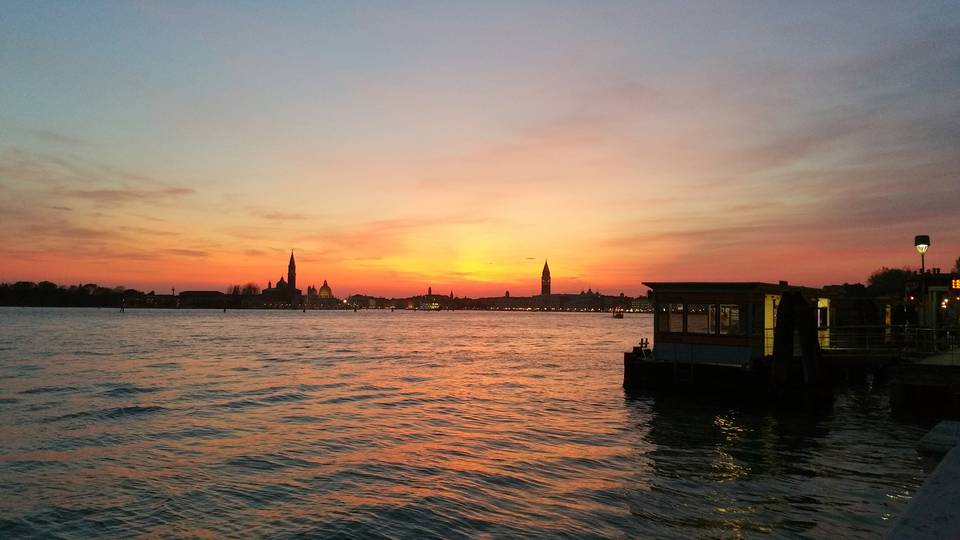
\includegraphics[width=\linewidth]{img/ccl/8.jpg}
        \end{frame}
\end{document}
